\graphicspath{{./figures}}

\section{Antennas}\label{sec:antenna_theory}

This section covers a very brief review of different types of antennas in literature, as well as how to practical feed these antennas with a transmission line, and a summary of their varying performances.

\subsection{Types}\label{sec:antenna_types}
There are various antenna types to consider for a satellite communication system. A highly customized design is out of the scope of this project, and therefore only designs with tunable parameters, or existing designs in literature, will be considered. Ultimately, each antenna's \textit{radiation pattern}, \textit{gain} (dBi i.e. decibels relative to an \textit{isotropic} source); fractional \textit{bandwidth}; main lobe \textit{beamwidth}; dimensions; and polarization will be compared. Here, \textit{polarization} refers to the orientation of the EM wave i.e. horizontal, vertical or circular.

\subsubsection{Half-Wavelength Dipole}

\begin{figure}[!htb]
  \begin{minipage}{.49\textwidth}
    \centering
    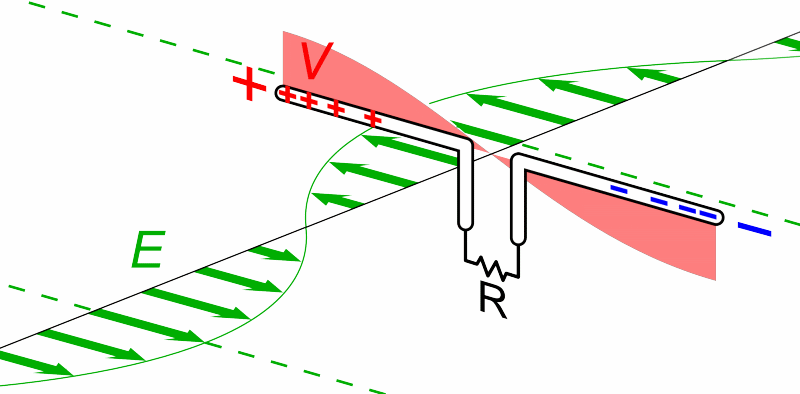
\includegraphics[width=0.8\linewidth]{dipole_geometry}
    \caption{Dipole Antenna Geometry}
    \label{fig:dipole_geometry}
  \end{minipage}
  \begin{minipage}{.49\textwidth}
    \centering
    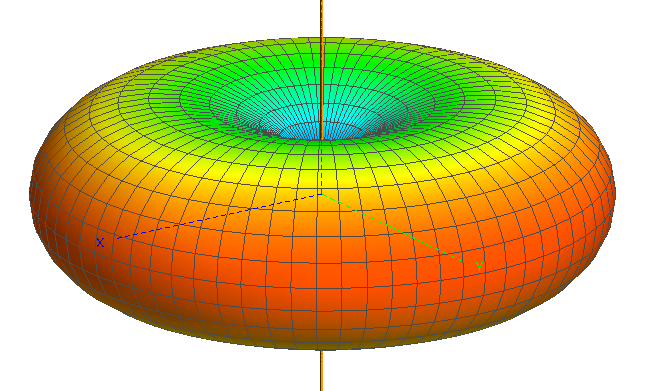
\includegraphics[width=0.6\linewidth]{dipole_pattern}
    \caption{Dipole Antenna Radiation Pattern}
    \label{fig:dipole_pattern}
  \end{minipage}
\end{figure}

The half-wavelength ($0.5 \lambda$) dipole anntenna is arguably the simplest and most common type of antenna. It consists of two conductive elements operating in opposite phase, as depicted in Figure \ref{fig:dipole_geometry}. It is described to have a donut-shaped radiation pattern as in Figure \ref{fig:dipole_pattern}, with \textit{omni-directional} radiation in the plane perpendicular to the conductor, and a \textit{null} tangential to the conductor. It has a maximum gain of 2.15 dBi, and is linearly polarized. \cite{site-antennaTheory}

\subsubsection{Quarter-Wave Monopole}\label{monopole}
The working principle of a monopole antenna makes use of the electromagnetic theory of \textit{imaging}. If an infinite ground plane or Perfect Electrical Conductor (PEC) is placed below one half of a $0.5 \lambda$ dipole antenna, since the PEC holds the constraint that the tangential electric field is zero across its boundary, an equal but opposite electromagnetic wave is ``induced" due to the incident wave. This wave ``appears" to have come from an equal but oppositely polarized ``image" source, hence removing the need for the second half of the dipole to be present.

These antennas are extremely useful when size is a constraint, however have the disadvantage of requiring a ground plane. A \textit{whip} antenna is a form of monopole antenna designed to be flexible so that it does not break as easily, and often without a ground plane with reduced performance. It is often placed inside a plastic enclosure, as in Figure \ref{fig:whip}. \cite{site-antennaTheory}

\begin{figure}[!htb]
  \begin{minipage}{.49\textwidth}
    \centering
    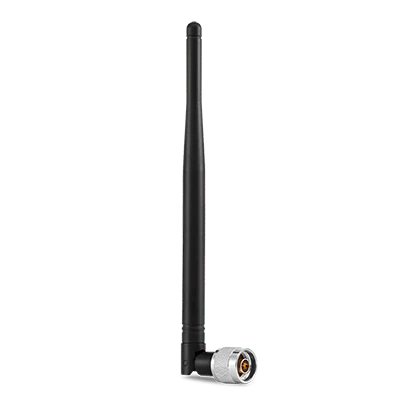
\includegraphics[width=0.6\linewidth]{whip}
    \caption{A Monopole Whip Antenna in a Plastic Housing}
    \label{fig:whip}
  \end{minipage}
  \begin{minipage}{.49\textwidth}
    \centering
    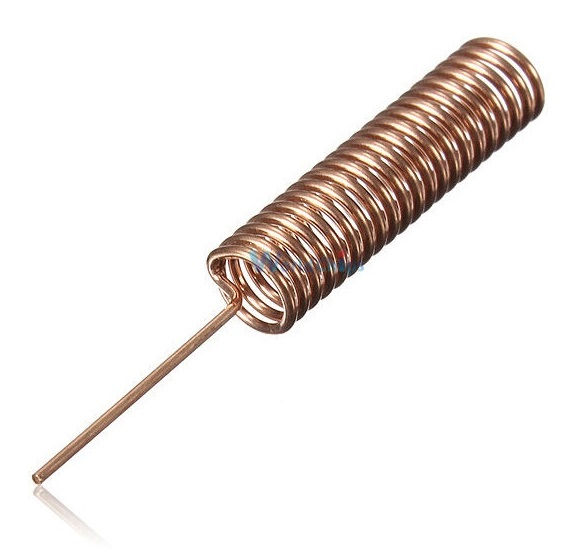
\includegraphics[width=0.6\linewidth]{helical_uni}
    \caption{A 21-turn Copper Helical Antenna}
    \label{fig:helical_uni}
  \end{minipage}
\end{figure}

\subsubsection{Helical}
Helical antennas are coiled windings of wire, where the circumference of the coil has some relationship with the desired frequency. Commonly, a circumference of $C = 1.0 \lambda$ is used for \textit{uni-directional} or \textit{axial mode} variants. In this case, a ground plane is required. The ground plane can also be \textit{cupped} (i.e. extended as an open cylinder) for additional directivity \cite{textbook-antennaTheoryAnalysisDesign}. \textit{Omni-directional} or \textit{normal mode} variants are possible without a ground plane, when $C << \lambda$. Figure \ref{fig:helical_uni} depicts a 21-turn example of such an antenna.

Helical antennas have several design parameters that influence the antenna's characteristics, such as number of turns ($n$), wire width ($wd$), and spacing between turns ($S$). A spacing of $0.20 \lambda < S < 0.25 \lambda$ is recommended, however smaller spacings of $0.10 \lambda < S < 0.20$ are commonly used \cite{site-helicalCalculator}. These antennas are also capable of either linear or circularly polarized signals. Lastly, since they can be designed with an arbitrarily small or large number of turns, and they have a large operating bandwidth, they can be made smaller than other alternatives.

\subsubsection{Patch}
A \textit{patch} or \textit{PCB} antenna is simply a rectangular PCB trace sized correctly to allow for radiation. Typically, a simple square or rectangular shape can be used. They allow for small profiles at the cost of efficiency \cite{site-antennaTheory}, and either have circular or linear polarization.

\subsubsection{Array}
In general, multiple antennas can be combined in an \textit{array} configuration. This allows complete manipulation of the design (such as the desired gain), by virtue of \textit{constructive} and \textit{destructive} interference of the electromagnetic waves. Common variations of this concept reside in \textit{Yagi-Uda} and \textit{Patch Array} antennas. \cite{site-antennaTheory}

\subsubsection{Yagi-Uda}
\begin{figure}[!htb]
  \begin{minipage}{.49\textwidth}
    \centering
    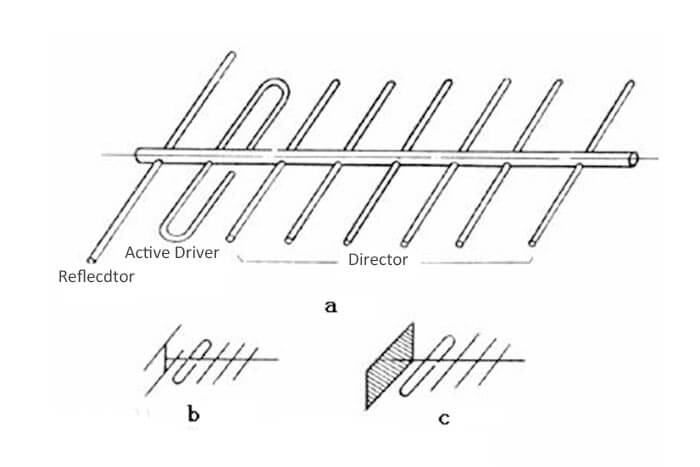
\includegraphics[width=0.8\linewidth]{yagi}
    \caption{Yagi-Uda Antenna Geometry \cite{site-icantennasYagi}}
    \label{fig:yagi}
  \end{minipage}
  \begin{minipage}{.49\textwidth}
    \centering
    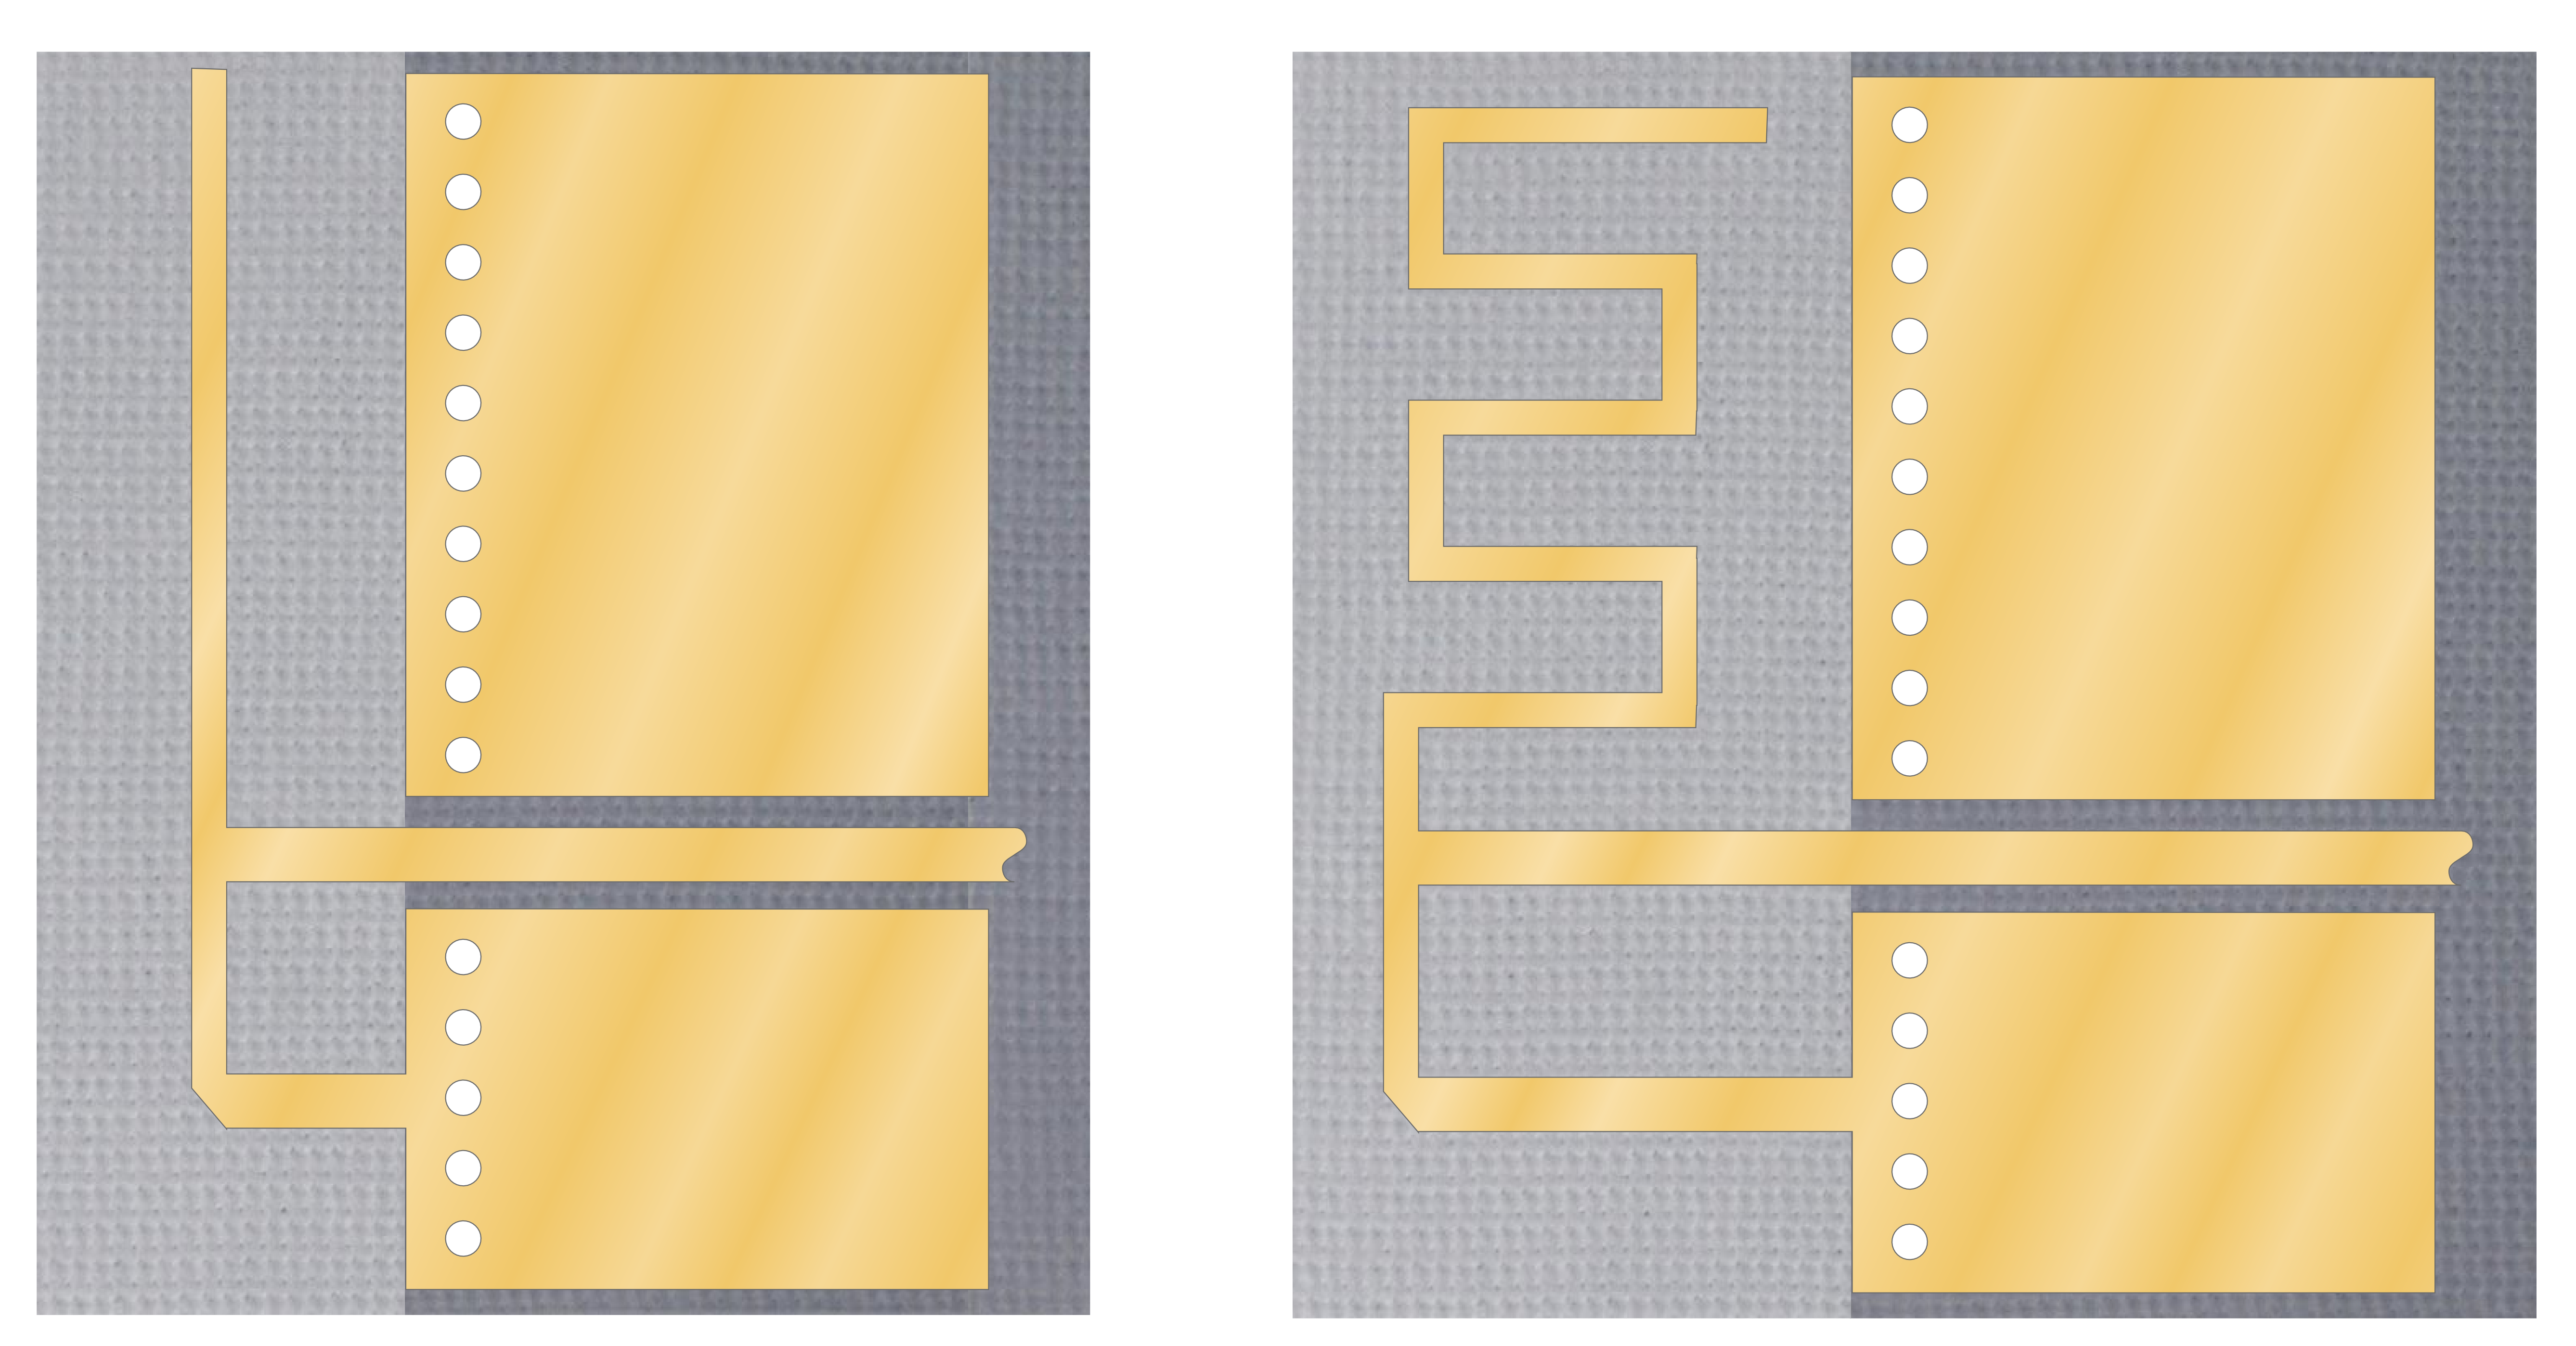
\includegraphics[width=0.8\linewidth]{invertedF}
    \caption{Two Inverted-F Microstrip Antenna Geometries \cite{site-invertedFAntenna}}
    \label{fig:invertedF}
  \end{minipage}
\end{figure}

Although not strictly an antenna array, \textit{Yagi-Uda} antennas are one of the most popular directive antennas that make use of interference. A given number of passive conductors are stacked in a specific configuration as show in Figure \ref{fig:yagi}, ultimately steering the EM waves using the concept of interference. Only one of the conductors in the array is fed with the signal. They generally can be made to have very large gain, and are linearly polarized. A \textit{cross-yagi} is a variation on this design which allows for circular polarization.

\subsubsection{Microstrip}
\textit{Microstrip} antennas generally refer to any planar, PCB antenna. They can be considered a generalization of a patch antenna. Many variations exist due to their flexible nature. A few examples include a: a \textit{patch array}; an \textit{inverted-F} design, which has a small form factor and a nearly 3D omni-directional radiation pattern; a \textit{ring antenna} \cite{paper-lowProfileRingAntenna}, which is uni-directional, and has an even smaller form factor than the inverted-F antenna; and a \textit{helical patch} antenna, which is simply a "zig-zag" helix shape flattened onto a PCB.

\subsection{Feedlines}
In general, \textit{feeding} an antenna is more complicated than simply connecting the amplifier's positive and negative terminals to the antenna's terminals. A $\SI{50}{\ohm}$ characteristic impedance is often used in RF systems. Since each antenna has a unique \textit{input impedance} which is generally different from this value, it must be \textit{matched} appropriately for optimal performance. A few well-known techniques for a number of the antennas in Section \ref{sec:antenna_types} are reviewed below.

\subsubsection{General}
A general, antenna-agnostic narrow-band technique for antenna impedance matching is to employ a "lumped element" matching circuit consisting mainly of inductors and capacitors. The most common example of this is an L-section, with exactly one capacitor and inductor.

\subsubsection{Half-Wavelength Dipole}
A half-wavelength dipole antenna has an input impedance of around $\SI{73}{\ohm}$, varying only due to the wire diameter used. A common method to reduce this impedance to $\SI{50}{\ohm}$ is simply to reduce the length of the dipole. In this case, a $\SI{50}{\ohm}$ match occurs from $\SI{0.42}{\lambda}$ to $\SI{0.44}{\lambda}$. \cite{textbook-antennaTheoryAnalysisDesign}

\subsubsection{Helical}\label{sec:helical_matching}
The input impedance of a helical antenna varies between 100 and 200 ohms. A common method to reduce this impedance is for the first quarter turn of the helix to be in the form of a conductive strip, and for the \textit{pitch angle} of this section to be close to zero \cite{textbook-antennaTheoryAnalysisDesign}. The height above the ground plane can then be varied to match the antenna appropriately, with the following equation approximately providing an approximate $\SI{50}{\ohm}$ match \cite{textbook-antennaTheoryAnalysisDesign}:
$$h = \frac{w}{\frac{377}{\sqrt{\epsilon_r} Z_0} - 2}$$

\subsection{Summary}
It is useful to have a qualitative comparison different antenna types as a reference for the design phase. This is presented in Table \ref{tab:antenna_characteristics} in the appendix, and has been tabulated using both the previous research, and general consensus in literature. Note that a \textit{narrow} beamwidth general corresponds to a \textit{uni-directional} antenna (and wide for omni-directional) and therefore this characteristic has not been included in the table.